\documentclass[9pt,english,,jou,floatsintext]{apa6}
\usepackage{lmodern}
\usepackage{amssymb,amsmath}
\usepackage{ifxetex,ifluatex}
\usepackage{fixltx2e} % provides \textsubscript
\ifnum 0\ifxetex 1\fi\ifluatex 1\fi=0 % if pdftex
  \usepackage[T1]{fontenc}
  \usepackage[utf8]{inputenc}
\else % if luatex or xelatex
  \ifxetex
    \usepackage{mathspec}
  \else
    \usepackage{fontspec}
  \fi
  \defaultfontfeatures{Ligatures=TeX,Scale=MatchLowercase}
\fi
% use upquote if available, for straight quotes in verbatim environments
\IfFileExists{upquote.sty}{\usepackage{upquote}}{}
% use microtype if available
\IfFileExists{microtype.sty}{%
\usepackage[]{microtype}
\UseMicrotypeSet[protrusion]{basicmath} % disable protrusion for tt fonts
}{}
\PassOptionsToPackage{hyphens}{url} % url is loaded by hyperref
\usepackage[unicode=true]{hyperref}
\hypersetup{
            pdftitle={Examining side effect variation of antipsychotic treatment in schizophrenia spectrum disorders},
            pdfborder={0 0 0},
            breaklinks=true}
\urlstyle{same}  % don't use monospace font for urls
\ifnum 0\ifxetex 1\fi\ifluatex 1\fi=0 % if pdftex
  \usepackage[shorthands=off,main=english]{babel}
\else
  \usepackage{polyglossia}
  \setmainlanguage[]{english}
\fi
\usepackage{longtable,booktabs}
% Fix footnotes in tables (requires footnote package)
\IfFileExists{footnote.sty}{\usepackage{footnote}\makesavenoteenv{long table}}{}
\usepackage{graphicx,grffile}
\makeatletter
\def\maxwidth{\ifdim\Gin@nat@width>\linewidth\linewidth\else\Gin@nat@width\fi}
\def\maxheight{\ifdim\Gin@nat@height>\textheight\textheight\else\Gin@nat@height\fi}
\makeatother
% Scale images if necessary, so that they will not overflow the page
% margins by default, and it is still possible to overwrite the defaults
% using explicit options in \includegraphics[width, height, ...]{}
\setkeys{Gin}{width=\maxwidth,height=\maxheight,keepaspectratio}
\IfFileExists{parskip.sty}{%
\usepackage{parskip}
}{% else
\setlength{\parindent}{0pt}
\setlength{\parskip}{6pt plus 2pt minus 1pt}
}
\setlength{\emergencystretch}{3em}  % prevent overfull lines
\providecommand{\tightlist}{%
  \setlength{\itemsep}{0pt}\setlength{\parskip}{0pt}}
\setcounter{secnumdepth}{0}

% set default figure placement to htbp
\makeatletter
\def\fps@figure{htbp}
\makeatother

% Manuscript styling
\usepackage{upgreek}
\captionsetup{font=singlespacing,justification=justified}

% Table formatting
\usepackage{longtable}
\usepackage{lscape}
% \usepackage[counterclockwise]{rotating}   % Landscape page setup for large tables
\usepackage{multirow}		% Table styling
\usepackage{tabularx}		% Control Column width
\usepackage[flushleft]{threeparttable}	% Allows for three part tables with a specified notes section
\usepackage{threeparttablex}            % Lets threeparttable work with longtable

% Create new environments so endfloat can handle them
% \newenvironment{ltable}
%   {\begin{landscape}\begin{center}\begin{threeparttable}}
%   {\end{threeparttable}\end{center}\end{landscape}}
\newenvironment{lltable}{\begin{landscape}\begin{center}\begin{ThreePartTable}}{\end{ThreePartTable}\end{center}\end{landscape}}

% Enables adjusting longtable caption width to table width
% Solution found at http://golatex.de/longtable-mit-caption-so-breit-wie-die-tabelle-t15767.html
\makeatletter
\newcommand\LastLTentrywidth{1em}
\newlength\longtablewidth
\setlength{\longtablewidth}{1in}
\newcommand{\getlongtablewidth}{\begingroup \ifcsname LT@\roman{LT@tables}\endcsname \global\longtablewidth=0pt \renewcommand{\LT@entry}[2]{\global\advance\longtablewidth by ##2\relax\gdef\LastLTentrywidth{##2}}\@nameuse{LT@\roman{LT@tables}} \fi \endgroup}

% \setlength{\parindent}{0.5in}
\setlength{\parskip}{0pt plus 0pt minus 0pt}

% \usepackage{etoolbox}
\makeatletter
\patchcmd{\HyOrg@maketitle}
  {\section{\normalfont\normalsize\abstractname}}
  {\section*{\normalfont\normalsize\abstractname}}
  {}{\typeout{Failed to patch abstract.}}
\makeatother
\shorttitle{Variation in side effects}
\leftheader{}
\author{Maria S. Neumeier\textsuperscript{1}, Stephanie Homan, Ph.D.\textsuperscript{1}, Stefan Vetter, M.D.\textsuperscript{1}, Erich Seifritz, M.D.\textsuperscript{1}, John M. Kane, M.D.\textsuperscript{2,3,4}, Maximilian Huhn, M.D.\textsuperscript{5}, Stefan Leucht, M.D.\textsuperscript{5}, \& Philipp Homan, M.D., Ph.D.\textsuperscript{1,2,3,4*}}
\affiliation{
\vspace{0.5cm}
\textsuperscript{1} University Hospital of Psychiatry Zurich, Zurich, Switzerland.\\\textsuperscript{2} Center for Psychiatric Neuroscience, Feinstein Institute for Medical Research, Manhasset, NY, USA.\\\textsuperscript{3} Division of Psychiatry Research, Zucker Hillside Hospital, Northwell Health, New York, NY, USA.\\\textsuperscript{4} Department of Psychiatry, Zucker School of Medicine at Northwell/Hofstra, Hempstead, NY, USA.\\\textsuperscript{5} Department of Psychiatry and Psychotherapy, Technical University of Munich, School of Medicine, Munich, Germany.}
\authornote{

Correspondence concerning this article should be addressed to Philipp Homan, M.D., Ph.D., University Hospital of Psychiatry Zurich, Lenggstrasse 31, 8032 Zurich, Switzerland. E-mail: philipp.homan@bli.uzh.ch}
\usepackage{dblfloatfix}


\usepackage{csquotes}
\usepackage{libertine}
\captionsetup[figure]{font=footnotesize,labelfont=bf}
\usepackage[printwatermark]{xwatermark}
\usepackage{xcolor}
\newcommand{\beginsupplement}{\setcounter{table}{0}  \renewcommand{\thetable}{S\arabic{table}} \setcounter{figure}{0} \renewcommand{\thefigure}{S\arabic{figure}}}

\title{Examining side effect variation of antipsychotic treatment in
schizophrenia spectrum disorders}

\date{}

\abstract{
Background: Side effects of antipsychotic drugs play a key role in
non-adherence and discontinuation of treatment in schizophrenia spectrum
disorders (SSD). Precision medicine aims to minimize such side effects
by selecting the right treatment for the right patient. However, to
determine the extent of precision medicine that is required, we need to
(1) show that there is indeed variation in side effects and (2) estimate
the amount of variation in those side effects between patients. While
clinical observations suggest that such variation may be considerable, a
statistical comparison of side effect variation between active and
control treatments is required to confirm this. Here, we hypothesized to
find larger side effect variation in treatment compared with control in
patients treated with first and second generation antipsychotics.
Methods: We included double-blind, placebo-controlled, randomized
controlled trials (RCTs) of adults with a diagnosis of SSD and
prescription for licensed antipsychotic drugs. Standard deviations of
the pre-post treatment differences of weight gain, prolactin levels, and
corrected QT (QTc) times were extracted. Data quality and validity were
ensured by following the PRISMA guidelines. The outcome measure was the
overall variability ratio of treatment to control across RCTs.
Individual variability ratios were weighted by the inverse-variance
method and entered into a random-effects model. Results: We included N =
16578 patients for weight gain, N = 16633 patients for prolactin levels,
and N = 10384 patients for QTc time. Variability ratios (VR) were
significantly increased for weight gain (VR = 1.08; 95\% CI: 1.02 -
1.14; P = 0.004) and prolactin levels (VR = 1.38; 95\% CI: 1.17 - 1.62;
P \textless{} 0.001) but did not reach significance for QTc time (VR =
1.05; 95\% CI: 0.98 - 1.12; P = 0.135). Conclusion: We found increased
variability in major side effects in patients with SSD under treatment
with second generation antipsychotics, suggesting that subgroups of
patients or even individual patients may benefit from improved treatment
allocation through stratified or personalized medicine, respectively.
}

\begin{document}
\maketitle

\section{Introduction}\label{introduction}

Antipsychotics are a fundamental component in the treatment of
schizophrenia spectrum disorders (SSD). Yet, a major problem are side
effects which play a key role in non-adherence and
discontinuation.\textsuperscript{1--5} A common hypothesis among
researchers and clinicians alike is that although side effects are
pervasive, not all patients are equally susceptible.\textsuperscript{6}
However, empirical support for this hypothesis is lacking, as randomized
controlled trials (RCTs) or conventional meta analyses by design cannot
answer whether such side effect variation does
exist.\textsuperscript{7,8}

To date, studies have established the efficacy, safety, and side effect
profiles of antipsychotic medications by averaging these indices across
groups of patients. Such studies can provide us with average side
effects, but they cannot tell us anything about individual patients or
subgroups.\textsuperscript{9,10} Nevertheless, before searching for
potential biomarkers that might predict individual susceptibility, we
should first quantify the extent to which such predictors are truly
needed.

An approach to answering this question is to shift the focus from the
means to the variances of side effects.\textsuperscript{11} By comparing
the variances between treatment and control groups of
RCTs,\textsuperscript{12} greater variability in treatment would
indicate that there is a component of variation, the side
effect-by-patient or side effect-by-subgroup interaction, that indicates
variability of side effects.\textsuperscript{11} Note that this
method\textsuperscript{13} has recently been applied for
antipsychotics,\textsuperscript{7}
antidepressants,\textsuperscript{8,14,15} and brain
stimulation.\textsuperscript{16} It is worth noting that these studies
found little evidence for treatment effect
variation.\textsuperscript{7,8,14,15} Importantly, in the case of
pre-post differences used as input for a meta-analysis of variance it is
crucial to think carefully about the way the variability ratio is
expressed,\textsuperscript{12,15,17} as the use of the coefficient of
variation ratio (CVR) that has been proposed as an alternative of the
variability ratio (VR)\textsuperscript{12} may lead to unreliable
results.\textsuperscript{13,17}

A recently published study investigated the individual treatment
response in antipsychotics and brought surprising
results.\textsuperscript{7,18} By comparing the variability between
treatment and control groups, no evidence was found for an increase in
variability in the treatment group. What might sound counter-intuitive
at first raises the question of how big the need for precision medicine
really is. However, that study evaluated the evidence for treatment
effect variation. It is possible that although such variation in
treatment effects is not as high as sometimes
assumed\textsuperscript{19}, it does exist in the susceptibility for
side effects. In other words, even if there is little variation in
response to treatment between patients, there may still be enough
variation in side effects to justify a need for precision medicine. If
true, then this would support optimization of treatment allocation with
respect to side effect profiles.\textsuperscript{20}

Side effects that are particularly relevant to antipsychotic treatment
include weight gain\textsuperscript{5}, hyperprolactinemia, and QTc
prolongation.\textsuperscript{20} Weight gain is a frequently observed
side effect that can negatively impact one's physical health and thus
may also influence treatment adherence. Every additional kilogram of
weight gain can contribute to an increased risk of heart
failure,\textsuperscript{21} cardiovascular
diesease,\textsuperscript{22} and diabetes.\textsuperscript{23} In
addition, treatment discontinuation is often seen in patients with
increase of weight under treatment.\textsuperscript{24} High prolactin
levels can lead to symptoms like decreased bone mass, gallactorhea, and
fertility problems in men and women. Further possible symptoms include
menstrual disturbances in female patients and decreased libido and
erectile dysfunction in male patients.\textsuperscript{25} These
symptoms are frequent, but often underreported by patients and unnoticed
as well as untreated by clinicians.\textsuperscript{26,27} They
furthermore might lead to loss in quality of life and might be a reason
for treatment discontinuation\textsuperscript{1,28} and subsequent
illness relapse, which together with persistent positive
symptoms\textsuperscript{29--32} may severly impact recovery and
therapeutic alliance.\textsuperscript{33} Prolongation of QTc was
observed in 7 of 14 antipsychotics compared by placebo in the intergroup
comparision by Huhn and colleagues.\textsuperscript{6} Importantly,
torsade de pointes tachycardia and sudden cardiac death are possible
severe consequences of QTc prolongation.\textsuperscript{34} Such
cardiac events are one of the factors that lead to the loss of life
expectancy observed in patients with SSD.\textsuperscript{35--37}

In summary, antipsychotic side effects are highly relevant for long-term
outcome and adherence in treatment of positive symptoms in SSD. The
question remains whether variability in side effects is high enough to
warrant efforts of treatment stratification or personalisation. Here, we
compared the variances of side effects including weight gain, prolactin
level and QTc-time between treatment and control groups to address this
question and to evaluate the evidence for the presence of side effect
variability. Based on the clinical impression that patients seem to vary
in their susceptibility to side effects, we hypothesized that the
variability in side effects would be higher in the treatment compared to
the control groups across all published trials of antipsychotics in
SSD.\textsuperscript{6}

\section{Methods}\label{methods}

\subsection{Search strategy and selection
criteria}\label{search-strategy-and-selection-criteria}

We used the data from the recent meta-analysis by Huhn and
colleagues.\textsuperscript{6} That study included placebo-controlled
published and unpublished trials investigating orally administered
atypical (second generation) antipsychotics and typical (first
generation) antipsychotics in adults with schizophrenia spectrum
disorders; and excluded patients with first episode psychosis, treatment
resistance, mainly negative symptoms, comorbidity with other mental or
physical illnesses and relapse-prevention studies. Long- and
short-acting intramuscular injections were also excluded (as they are
often used in relapse prevention or emergency treatment) and studies
from mainland China were excluded because of data quality
concerns.\textsuperscript{38} Data sources were MEDLINE, Cochrane
Central Register of Controlled Trials (CENTRAL), Embase, Biosis,
PsycINFO, PubMed, ClinicalTrials.gov, WHO International Clinical Trials
Registry Platform and the US Food and Drug Administration until January
8 2019. Data quality and validity were ensured by following the PRISMA
guidelines.\textsuperscript{39} For missing data, we also contacted
study authors.

For the analysis, we used the standard deviations of pre-post
differences in side effects. The primary outcome was the overall
variability ratio of side effects in treatment versus control groups.
Standard deviations (SD) and number of patients (N) were extracted for
weight gain, prolactin level and QTc time. The units used were kg for
weight gain, ng/mL for prolactin levels, and ms for QTc time. Some
studies provided data for all of the three side effects, whereas the
majority of the studies contained less data (see Results).

\subsection{Statistical analysis}\label{statistical-analysis}

If patients or subgroups differ in their susceptibility to side effects,
we would expect to observe increased variances in the treatment-
compared with the control group. To test this, we computed the log
variability ratio (log VR) by comparing the relative variability of side
effects under treatment versus control:

\[\textrm{log VR}=\textrm{log}\left(\frac{\textrm{SD}_{\textrm{Tx}}}{\textrm{SD}_{\textrm{Ct}}} \right) +
\frac{1}{2(n_{\textrm{Tx}}-1)} - \frac{1}{2(n_{\textrm{Ct}}-1)} \],

where \(\textrm{SD}_{\textrm{Tx}}\) was the reported sample SD for side
effects under treatment, \(\textrm{SD}_{\textrm{Ct}}\) was the reported
sample SD for side effects under control, \(n_{\textrm{Tx}}\) was the
treatment sample size, and \(n_{\textrm{Ct}}\) the control sample size.
The corresponding sampling variance (\(s_{\textrm{log VR}}^2\)) for each
comparison can be expressed as follows:

\[ s_{\textrm{log VR}}^2 = \frac{1}{2(n_{\textrm{Tx}}-1)} + \frac{1}{2(n_{\textrm{Ct}}-1)}\].

The individual variability ratios were weighted with the inverse of this
sampling variance\textsuperscript{40} and entered into a random-effects
model to quantify the overall variability ratio of side effects. For
better interpretability, results were back-transformed from the
logarithmic scale. Here, a variability ratio greater than one would
indicate a higher side effect variability in treatment compared to
control, whereas a variability ratio smaller than one indicates less
side effect variability under treatment compared with control.

\subsection{Data and code
availability}\label{data-and-code-availability}

The analysis was performed from September 2019 to May 2020, using the R
package metafor\textsuperscript{40}(version 2.1.0). The manuscript was
produced with the R packages rmarkdown (version 2.1); represearch
(version 0.0.0.9000; \url{https://github.com/phoman/represearch/});
knitr (version 1.26); and papaja (version 0.1.0.9942). All data and code
are freely available online to ensure reproducibility at
\url{https://github.com/homanlab/sideeffects/}.

\section{Results}\label{results}

\subsection{Overall reporting details}\label{overall-reporting-details}

Together, we screened N = 151 studies from the original meta-analysis by
Huhn and colleagues\textsuperscript{6} as these studies reported data on
at least one of the three side effects that we were interested in. Of
these studies, N = 94 (62\%) had missing variance measures despite
reported means for at least one of the three side effects. We thus
included the N = 60 (40\%) studies that did report variance measures for
at least one of the side effects of interest.

\subsection{Weight gain}\label{weight-gain}

For weight gain, we included 51 RCTs, yielding 72 comparisons of
antipsychotic drugs with placebo to investigate the individual
occurrence of weight gain in patients. All together we included N =
16578 patients diagnosed with schizophrenia or schizoaffective disorder.
There were 11373 (69\%) patients randomly allocated to the treatment
group, and 5205 (31\%) to the placebo group. Overall, the variability
for weight gain was higher under treatment than under control (VR =
1.08; 95\% CI: 1.02 - 1.14; P = 0.004; Figure \ref{fig:fig1}).
Individual comparisons between drugs across studies indicated marked
differences between individual antipsychotics (VR = 1.08; 95\% CI: 1.02
- 1.14; P = 0.004; Figure \ref{fig:fig2}).

\begin{figure}
\centering
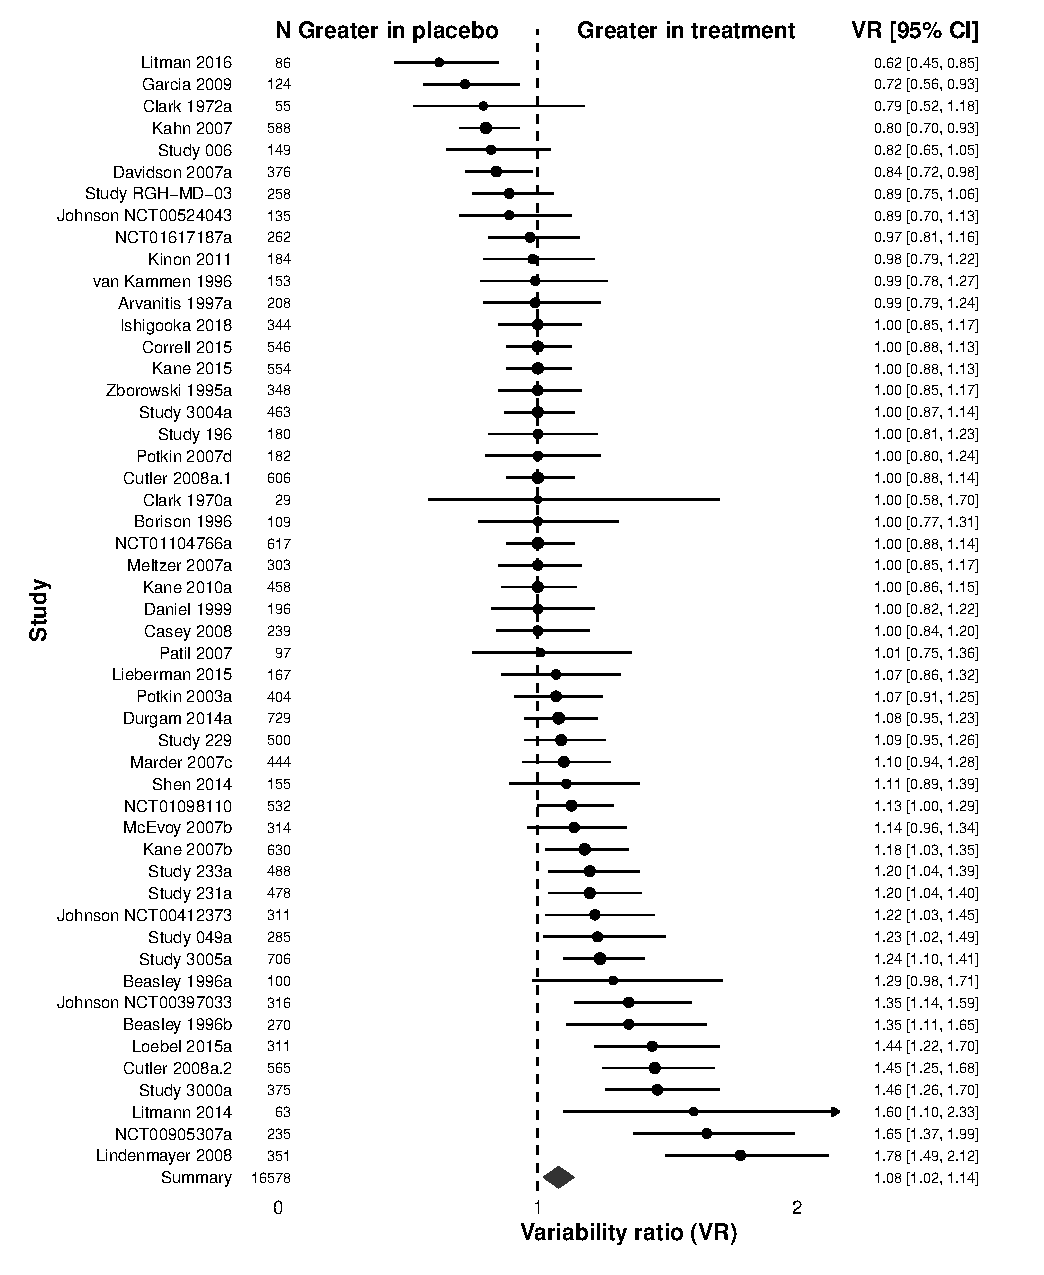
\includegraphics{../output/figures/weightsd_fig1.pdf}
\caption{\label{fig:fig1}Variability ratio for weight gain. The forest plot
shows the VR together with its 95\% confidence interval (CI) for
treatment versus control. All included studies\textsuperscript{41--93}
are also listed in Table S1.}
\end{figure}

\begin{figure}
\centering
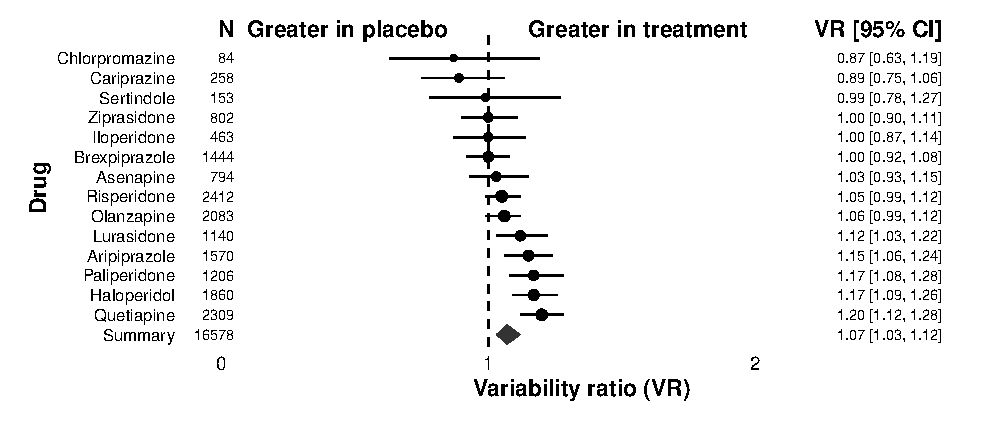
\includegraphics{../output/figures/weightsd_fig2.pdf}
\caption{\label{fig:fig2}Variability ratio for weight gain for individual
antipsychotics. The forest plot shows the VR together with its 95\%
confidence interval (CI) for treatment versus control. All included
studies\textsuperscript{41--93} are also listed in Table S1.}
\end{figure}

\subsection{Hyperprolactinemia}\label{hyperprolactinemia}

For hyperprolactinemia, we included 50 RCTs, with 71 comparisons of
antipsychotic drugs with placebo. All together we included N = 16633
patients diagnosed with schizophrenia or schizoaffective disorder. There
were 11409 (69\%) patients randomly allocated to the treatment group,
and 5224 (31\%) to the placebo group. Overall, the variability for
hyperprolactinemia was higher under treatment than under control (VR =
1.38; 95\% CI: 1.17 - 1.62; P \textless{} 0.001; Figure \ref{fig:fig3}).
Individual comparisons between drugs across studies indicated marked
differences between individual antipsychotics (VR = 1.38; 95\% CI: 1.17
- 1.62; P \textless{} 0.001; Figure \ref{fig:fig4}).

\begin{figure}
\centering
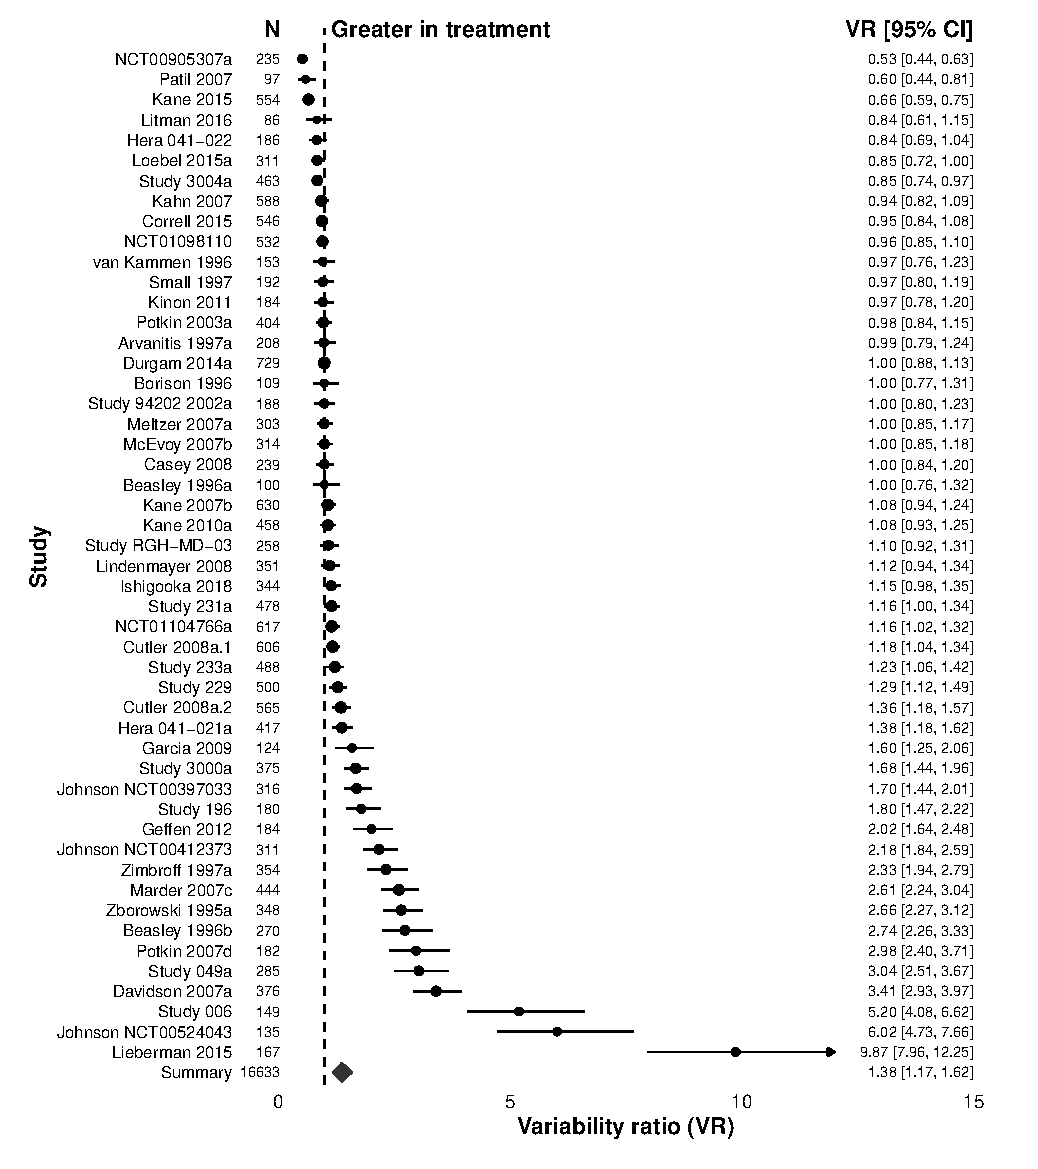
\includegraphics{../output/figures/prolactinsd_fig1.pdf}
\caption{\label{fig:fig3}Variability ratio for hyperprolactinemia. The
forest plot shows the VR together with its 95\% confidence interval (CI)
for treatment versus control. All included
studies\textsuperscript{41,42,44--48,50--58,60,62,64,65,67--69,72,74--79,82--90,92--100}
are also listed in Table S1.}
\end{figure}

\begin{figure}
\centering
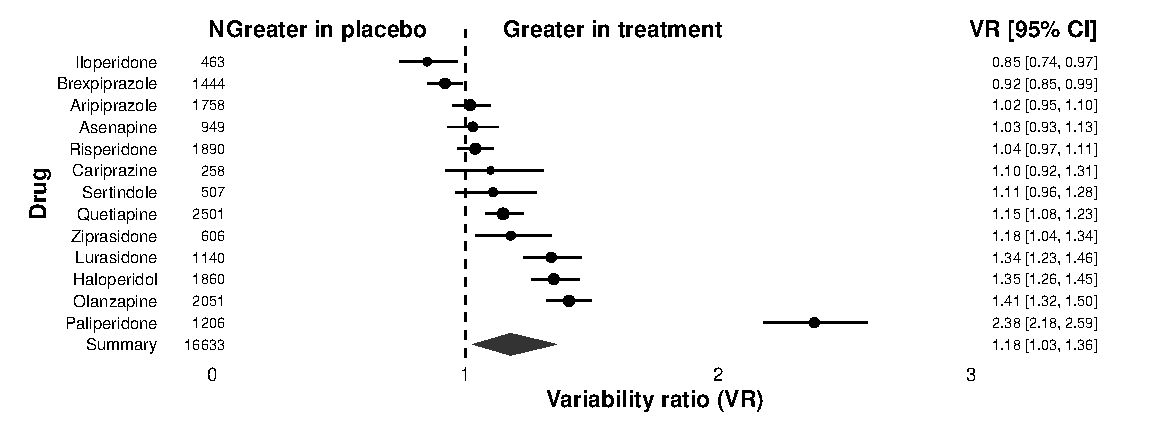
\includegraphics{../output/figures/prolactinsd_fig2.pdf}
\caption{\label{fig:fig4}Variability ratio for hyperprolactinemia for
individual antipsychotics. The forest plot shows the VR together with
its 95\% confidence interval (CI) for treatment versus control. All
included
studies\textsuperscript{41,42,44--48,50--58,60,62,64,65,67--69,72,74--79,82--90,92--100}
are also listed in Table S1.}
\end{figure}

\subsection{QTc prolongation}\label{qtc-prolongation}

For QTc prolongation, we included 29 RCTs, with 46 comparisons of
antipsychotic drugs with placebo. All together we included N = 10384
patients diagnosed with schizophrenia or schizoaffective disorder. There
were 7439 (72\%) patients randomly allocated to the treatment group, and
2945 (28.00\%) to the placebo group. Even though the variability for QTc
prolongation was higher under treatment than under control, the
difference did not reach statistical significance (VR = 1.05; 95\% CI:
0.98 - 1.12; P = 0.135; Figure \ref{fig:fig5}).

However, individual comparisons between drugs across studies indicated
marked differences between individual antipsychotics, with sertindole
and haloperidol leading to significant increases in variability compared
to control (VR = 1.05; 95\% CI: 0.98 - 1.12; P = 0.135; Figure
\ref{fig:fig6}).

\begin{figure}
\centering
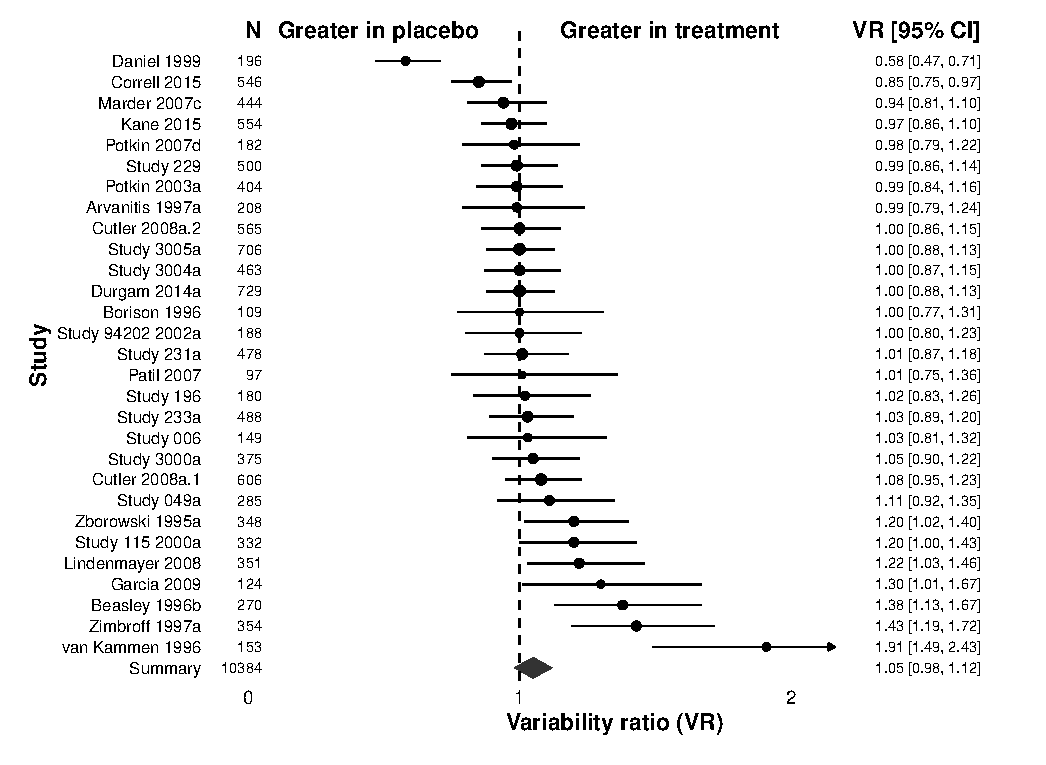
\includegraphics{../output/figures/qtcsd_fig1.pdf}
\caption{\label{fig:fig5}Variability ratio for QTc prolongation. The forest
plot shows the VR together with its 95\% confidence interval (CI) for
treatment versus control. All included
studies\textsuperscript{42,45,51,52,54--60,62,68,70,74,76--80,85,86,89,93,94,99,100}
are also listed in Table S1.}
\end{figure}

\begin{figure}
\centering
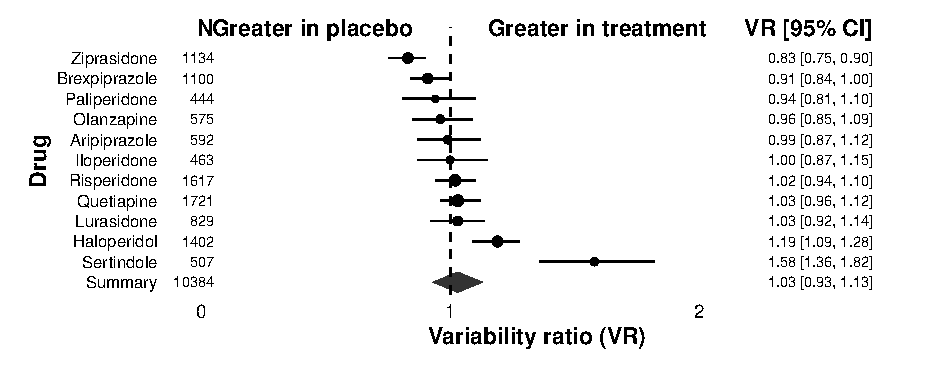
\includegraphics{../output/figures/qtcsd_fig2.pdf}
\caption{\label{fig:fig6}Variability ratio for QTC prolongation for
individual antipsychotics. The forest plot shows the VR together with
its 95\% confidence interval (CI) for treatment versus control. All
included
studies\textsuperscript{42,45,51,52,54--60,62,68,70,74,76--80,85,86,89,93,94,99,100}
are also listed in Table S1.}
\end{figure}

\section{Discussion}\label{discussion}

\subsection{Summary}\label{summary}

This study assessed the variability in the three major side effects of
antipsychotic treatment in schizophrenia spectrum disorders. We focused
on side effects because their occurrence has a great impact on treatment
adherence and pyhsical health of patients, and clinical experience
suggests a potential to improve treatment allocation by taking into
account the variability in side effect occurrence. We wanted to quantify
the evidence in support of this experience, relevant for clinicians as
much as for translational researchers. We also know from clinical trials
and meta-analyses that some antipsychotics are more associated with
specific side effects than others. For example, clozapine and olanzapine
are strongly associated with weight gain,\textsuperscript{6,20,101}
QTc-time prolongation is most distinct in sertindole and
amisulpride\textsuperscript{6}, and prolactin level elevation in
paliperidone and risperidone.\textsuperscript{6} However, these data
cannot address the question whether there is variability in subgroups or
individual patients. Such side effect-by-subgroup or side
effect-by-patient interaction would be a prime example for the need of a
more stratified or personalized medicine, respectively, which allocates
treatments according to side effect profiles of subgroups or individual
patients. The presence of such subgroups or individual patients would
result in an increase of the side effect variability of treated patients
compared to those who received placebo.\textsuperscript{7,13}. The
amount of this increase can be captured by the variability ratio (VR)
which compares the variability of treatment versus control for each side
effect. Evaluating all studies that reported variance measures for at
least one of the investigated side effects,\textsuperscript{6} we found
that the reporting of standard deviations was often incomplete. In terms
of variability of side effects, we found that the variability for weight
gain and prolactin elevation was indeed significantly increased in
patients who received treatment compared to those who received placebo.
For QTc prolongation, this increase was did not reach significance.
Together, our results suggest that there is indeed marked variability in
the occurrence of side effects in antipsychotic treatment.

\subsection{Reporting}\label{reporting}

Altogether we included 43595 patients from 60 studies. Only for about
40\% of studies included in a previous meta-analysis\textsuperscript{6}
variance data for at least one of the side effects of interest (weight
gain, prolactin levels, QTc prolongation) were available. In about 62\%
of the studies included\textsuperscript{6} incomplete data existed such
that means were reported without a measure of variance. Although we did
contact authors for missing data whenever possible, we received missing
data only for three studies. In summary, consistent reporting of
antipsychotic side effects, specifically with respect to variability
measures, is currently missing in the literature and should be improved
in future studies.

\subsection{Weight gain}\label{weight-gain-1}

Weight gain in antipsychotics, especially in second generation
antipsychotics,\textsuperscript{102} is a severe side effect that can
contribute to metabolic dysregulation. Importantly, every kg of weight
gain leads to a linear increase in the risk of cardiovascular
diseases\textsuperscript{22}, heart failure\textsuperscript{21}, and
diabetes\textsuperscript{23}. Clozapine, olanzapine, zotepine and
sertindole have the most severe impact in gaining weight. Some studies
showed that a lower BMI at baseline\textsuperscript{103} and
sex\textsuperscript{104} can lead to more weight gain, whereas other
studies found that male sex and higher BMI at baseline are related to a
higher risk of metabolic distrubances.\textsuperscript{20} Our findings
provide evidence that some patients are indeed more susceptible to
antipsychotic weight gain than others. As antipsychotics in the
treatment for schizophrenia and related diseases is often recommended to
be taken as a relapse prevention for a longer
period,\textsuperscript{105,106} patients are likely to gain more weight
during their treatment over months and years. Together, this suggests
that there is a potential to improve long-term health and adherence by
identifying the subgroups or individual patients that are particularly
prone to weight gain. Preliminary evidence suggests that a dysregulated
striatal reward circuit contributes to weight gain
susceptbility.\textsuperscript{5,107}

\subsection{Hyperprolactinemia}\label{hyperprolactinemia-1}

Prolactin level elevations occur in up to 70\% of
patients\textsuperscript{108} under the treatment with antipsychotic
drugs. By blocking dopamine D2 receptors on lacotroph cells a
disinhibition of the synthesis and secretion of prolactin is
observed.\textsuperscript{109,110} This can lead to both, short- and
long-term side effects with potentially severe impact on our patients
health. Typical short time effects include galactorrhea, gynecomastia,
menstrual irregularities, and sexual dysfunction; a typical long-term
result is osteoporosis.\textsuperscript{111,112} and a potentially
increased risk in developing breast cancer in association with
hyperprolactinemia.\textsuperscript{113,114} Our findings suggest that
these risks may be particularly relevant for some patients but not other
patients. For example, a previous study found that prolactin level
elevations are more pronounced and more frequent in women than in
men.\textsuperscript{115} In addition, some antipsychotics such as
amisulprid, risperidone, and paliperidone are linked to a greater
elevation of prolactin.\textsuperscript{6,115} In summary, and in line
with the weight gain findings, this suggests that there is a potential
to improve long-term health and antipsychotic adherence by identifying
the subgroups or individual patients that are particularly likely to
develop prolactine elevations under antipsychotic treatment.

\subsection{QTc prolongation}\label{qtc-prolongation-1}

Prolongation of QTc is another important antipsychotic side effect as
cardiovascular diseases remain the most common cause of natural
mortality in schizophrenia spectrum disorders.\textsuperscript{116}
Users of antipsychotic medication are reported to have higher rates of
sudden cardiac death than nonusers.\textsuperscript{117} Prolongation of
QTc (longer than 450 ms in men and longer than 470 ms in women,
respectively, when corrected with Bazetts Formula\textsuperscript{118})
can contribute to this.\textsuperscript{34} A prolongation of QTc can
lead to torsade de pointes and subsequently to sudden
death.\textsuperscript{119,120} The molecular pathway of this side
effect is not completely understood.\textsuperscript{121} It is known,
however, that some medications such as sertindole, amisulprid,
ziprasidone lead to more QTc prolongation than
others.\textsuperscript{6} Our findings suggest that although QTc
prolongation varies between subgroups or patients this increased
variability is not statistically significant, potentially because of a
smaller number of studies available which decreased the statistical
power. Previous studies suggest that risk factors may include female
sex, comorbid cardiovascular disease, high drug dosages, and electrolyte
disturbances.\textsuperscript{122}

\subsection{Limitations and strengths}\label{limitations-and-strengths}

Our meta-analysis had some limitations. First, the occurrence of side
effects might be a dosage dependent effect, which could reflect a
higher/different VR in some studies. Second, the level of prolactin can
be highly variable based on multiple biological and methodological
factors such as stress, diurnal variation and type of assay performed.
This might explain the surprising difference in prolactin level
variability between risperidone and paliperidone, two highly similar
drugs. Third, for QTc, a reduced number of studies was available,
potentially reducing statistical power to detect a significant
variability increase. Finally, our method cannot determine whether the
increased variability is due to variability differences in subgroups or
individual patients.\textsuperscript{11}. The particular strength of our
study is that we included all available studies of antipsychotic
treatment in SSD reporting variability measures for side effects of
interest. To our knowledge, this is the first comprehensive study that
provides evidence for substantial variability in side effects.

\subsection{Conclusion}\label{conclusion}

Our findings suggest that there is enough variability in two major side
effects (weight gain and prolactin elevation) to assume that subgroups
of patients or even individual patients may benefit from improved
treatment allocation through stratified or personalized medicine,
respectively. Such efforts in precision medicine might be crucial to
improve adherence\textsuperscript{123} and long-term health under
antipsychotic treatment.

\section{Acknowledgements}\label{acknowledgements}

The authors thank Majnu John, PhD, for advice on the analysis of the
current study and Ellen Ji, PhD, for her thoughtful comments on the
manuscript. These individuals received no additional compensation,
outside of their usual salary, for their contributions.

\section{Funding/Support}\label{fundingsupport}

PH is supported by a NARSAD grant from the Brain \& Behavior Research
Foundation (28445) and by a Research Grant from the Novartis Foundation
(20A058).

\section{Conflict of interest}\label{conflict-of-interest}

In the last 3 years Dr.~Leucht has received honoraria for service as a
consultant or adviser and/or for lectures from Angelini, Böhringer
Ingelheim, Geodon\&Richter, Janssen, Johnson\&Johnson, Lundbeck, LTS
Lohmann, MSD, Otsuka, Recordati, SanofiAventis, Sandoz, Sunovion, TEVA.
Dr.~Kane reported grants from Otsuka, Lundbeck and Janssen, as well as
other from Alkermes, Allergan, Forum, Genentech, Lundbeck, Intracellular
Therapies, Janssen, Johnson \& Johnson, Merck, Neurocrine, Otsuka,
Pierre Fabre, Reviva, Roche, Sunovion, Takeda, Teva, Vanguard Research
Group, and LB Pharmaceuticals outside of the submitted work. No other
disclosures were reported.

\section{References}\label{references}

\hypertarget{refs}{}
\hypertarget{ref-Lambert2004}{}
1. Lambert, M. \emph{et al.} Impact of present and past antipsychotic
side effects on attitude toward typical antipsychotic treatment and
adherence. \emph{European Psychiatry} \textbf{19}, 415--422 (2004).

\hypertarget{ref-Kane2013}{}
2. Kane, J. M., Kishimoto, T. \& Correll, C. U. Non-adherence to
medication in patients with psychotic disorders: Epidemiology,
contributing factors and management strategies. \emph{World Psychiatry}
\textbf{12}, 216--226 (2013).

\hypertarget{ref-Sendt2015}{}
3. Sendt, K.-V., Tracy, D. K. \& Bhattacharyya, S. A systematic review
of factors influencing adherence to antipsychotic medication in
schizophrenia-spectrum disorders. \emph{Psychiatry Research}
\textbf{225}, 14--30 (2015).

\hypertarget{ref-Wade2017}{}
4. Wade, M., Tai, S., Awenat, Y. \& Haddock, G. A systematic review of
service-user reasons for adherence and nonadherence to neuroleptic
medication in psychosis. \emph{Clinical Psychology Review} \textbf{51},
75--95 (2017).

\hypertarget{ref-Homan2019k}{}
5. Homan, P. \emph{et al.} Striatal volume and functional connectivity
correlate with weight gain in early-phase psychosis.
\emph{Neuropsychopharmacology} (2019).

\hypertarget{ref-Huhn2019}{}
6. Huhn, M. \emph{et al.} Comparative efficacy and tolerability of 32
oral antipsychotics for the acute treatment of adults with multi-episode
schizophrenia: A systematic review and network meta-analysis. \emph{The
Lancet} \textbf{394}, 939--951 (2019).

\hypertarget{ref-Winkelbeiner2019}{}
7. Winkelbeiner, S., Leucht, S., Kane, J. M. \& Homan, P. Evaluation of
Differences in Individual Treatment Response in Schizophrenia Spectrum
Disorders: A Meta-analysis. \emph{JAMA Psychiatry} (2019)
doi:\href{https://doi.org/10.1001/jamapsychiatry.2019.1530}{10.1001/jamapsychiatry.2019.1530}.

\hypertarget{ref-Munkholm2019}{}
8. Munkholm, K., Winkelbeiner, S. \& Homan, P. Individual response to
antidepressants for depression in adults - a simulation study and
meta-analysis. \emph{PsyArXiv} (2019)
doi:\href{https://doi.org/10.31219/osf.io/srzx5}{10.31219/osf.io/srzx5}.

\hypertarget{ref-Senn2016}{}
9. Senn, S. Mastering variation: Variance components and personalised
medicine. \emph{Statistics in Medicine} \textbf{35}, 966--977 (2016).

\hypertarget{ref-Senn2018}{}
10. Senn, S. Statistical pitfalls of personalized medicine.
\emph{Nature} \textbf{563}, 619--621 (2018).

\hypertarget{ref-Cortes2019}{}
11. Cortés, J. \emph{et al.} Does evidence support the high expectations
placed in precision medicine? A bibliographic review. \emph{F1000
Research} \textbf{7}, (2019).

\hypertarget{ref-Nakagawa2015}{}
12. Nakagawa, S. \emph{et al.} Meta-analysis of variation: Ecological
and evolutionary applications and beyond. \emph{Methods in Ecology and
Evolution} \textbf{6}, 143--152 (2015).

\hypertarget{ref-Mills2020}{}
13. Mills, H. L. \emph{et al.} Detecting heterogeneity of intervention
effects using analysis and meta-analysis of differences in variance
between arms of a trial. \emph{MedRxiv} (2020)
doi:\href{https://doi.org/10.1101/2020.03.07.20032516}{10.1101/2020.03.07.20032516}.

\hypertarget{ref-Ploderl2019}{}
14. Plöderl, M. \& Hengartner, M. P. What are the chances for
personalised treatment with antidepressants? Detection of
patient-by-treatment interaction with a variance ratio meta-analysis.
\emph{BMJ Open} \textbf{9}, (2019).

\hypertarget{ref-Volkmann2020}{}
15. Volkmann, C. M. D., Volkmann, A. \& Mueller, C. On the treatment
effect heterogeneity of antidepressants in major depression. a bayesian
meta-analysis. \emph{MedRxiv} (2020).

\hypertarget{ref-Winkelbeiner2020}{}
16. Winkelbeiner, S. \emph{et al.} Treatment effect variation in brain
stimulation across psychiatric disorders. \emph{MedRxiv} (2020)
doi:\href{https://doi.org/10.1101/2020.05.02.20088831}{10.1101/2020.05.02.20088831}.

\hypertarget{ref-Volkmann2020a}{}
17. Volkmann, A. On the relationship between treatment effect
heterogeneity and the variability ratio effect size statistic.
\emph{arXiv} (2020).

\hypertarget{ref-Winkelbeiner2019b}{}
18. Winkelbeiner, S. \& Homan, P. Is variance ratio a valid indicator of
heterogeneous treatment effect?-reply. \emph{JAMA Psychiatry} (2019)
doi:\href{https://doi.org/10.1001/jamapsychiatry.2019.3382}{10.1001/jamapsychiatry.2019.3382}.

\hypertarget{ref-Homan2019a}{}
19. Homan, P. \emph{et al.} Structural similarity networks predict
clinical outcome in early-phase psychosis.
\emph{Neuropsychopharmacology} \textbf{44}, 915--922 (2019).

\hypertarget{ref-Pillinger2020}{}
20. Pillinger, T. \emph{et al.} Comparative effects of 18 antipsychotics
on metabolic function in patients with schizophrenia, predictors of
metabolic dysregulation, and association with psychopathology: A
systematic review and network meta-analysis. \emph{The Lancet
Psychiatry} \textbf{7}, 64--77 (2020).

\hypertarget{ref-Kenchaiah2002}{}
21. Kenchaiah, S. \emph{et al.} Obesity and the risk of heart failure.
\emph{New England Journal of Medicine} \textbf{347}, 305--313 (2002).

\hypertarget{ref-Willett1995}{}
22. Willett, W. C. \emph{et al.} Weight, weight change, and coronary
heart disease in women. Risk within the 'normal' weight range.
\emph{JAMA} \textbf{273}, 461--465 (1995).

\hypertarget{ref-Cooper2016}{}
23. Cooper, S. J. \emph{et al.} BAP guidelines on the management of
weight gain, metabolic disturbances and cardiovascular risk associated
with psychosis and antipsychotic drug treatment. \emph{Journal of
Psychopharmacology} \textbf{30}, 717--748 (2016).

\hypertarget{ref-Mustafa2018}{}
24. Mustafa, S. \emph{et al.} Predictors of `all-cause
discontinuation'of initial oral antipsychotic medication in first
episode psychosis. \emph{Schizophrenia Research} \textbf{201}, 287--293
(2018).

\hypertarget{ref-Thapa2020}{}
25. Thapa, S. \& Bhusal, K. Hyperprolactinemia. in \emph{StatPearls}
(StatPearls Publishing, 2020).

\hypertarget{ref-Montejo2010}{}
26. Montejo, Á. L. \emph{et al.} Frequency of sexual dysfunction in
patients with a psychotic disorder receiving antipsychotics.
\emph{Journal of Sexual Medicine} \textbf{7}, 3404--3413 (2010).

\hypertarget{ref-Serretti2011}{}
27. Serretti, A. \& Chiesa, A. A meta-analysis of sexual dysfunction in
psychiatric patients taking antipsychotics. \emph{International Clinical
Psychopharmacology} \textbf{26}, 130--140 (2011).

\hypertarget{ref-Heald2010}{}
28. Heald, A. Physical health in schizophrenia: A challenge for
antipsychotic therapy. \emph{European Psychiatry} \textbf{25}, S6--S11
(2010).

\hypertarget{ref-Homan2012a}{}
29. Homan, P., Kindler, J., Hauf, M., Hubl, D. \& Dierks, T. Cerebral
blood flow identifies responders to transcranial magnetic stimulation in
auditory verbal hallucinations. \emph{Translational Psychiatry}
\textbf{2}, e189 (2012).

\hypertarget{ref-Cavelti2018}{}
30. Cavelti, M. \emph{et al.} Neuroimaging of formal thought disorder in
schizophrenia: A systematic review. \emph{Schizoprenia Research} 2--16
(2018).

\hypertarget{ref-Cavelti2018a}{}
31. Cavelti, M. \emph{et al.} Formal thought disorder is related to
aberrations in language-related white matter tracts in patients with
schizophrenia. \emph{Psychiatry Research: Neuroimaging} 40--50 (2018).

\hypertarget{ref-Winkelbeiner2018a}{}
32. Winkelbeiner, S. \emph{et al.} Decreased blood flow in the right
insula and middle temporal gyrus predicts negative formal thought
disorder in schizophrenia. \emph{Schizophrenia Research} \textbf{201},
432--434 (2018).

\hypertarget{ref-Cavelti2016}{}
33. Cavelti, M., Homan, P. \& Vauth, R. The impact of thought disorder
on therapeutic alliance and personal recovery in schizophrenia and
schizoaffective disorder: An exploratory study. \emph{Psychiatry
Research} \textbf{239}, 92--98 (2016).

\hypertarget{ref-Funk2020}{}
34. Funk, M. C. \emph{et al.} QTc prolongation and psychotropic
medications. \emph{The American Journal of Psychiatry} \textbf{177},
273--274 (2020).

\hypertarget{ref-Glassman2005}{}
35. Glassman, A. H. Schizophrenia, antipsychotic drugs, and
cardiovascular disease. \emph{Journal of Clinical Psychiatry}
\textbf{66}, 5--10 (2005).

\hypertarget{ref-Vandael2017}{}
36. Vandael, E., Vandenberk, B., Vandenberghe, J., Willems, R. \&
Foulon, V. Risk factors for qtc-prolongation: Systematic review of the
evidence. \emph{International Journal of Clinical Pharmacy} \textbf{39},
16--25 (2017).

\hypertarget{ref-Koponen2008}{}
37. Koponen, H. \emph{et al.} Schizophrenia and sudden cardiac death---a
review. \emph{Nordic Journal of Psychiatry} \textbf{62}, 342--345
(2008).

\hypertarget{ref-Tong2018}{}
38. Tong, Z., Li, F., Ogawa, Y., Watanabe, N. \& Furukawa, T. A. Quality
of randomized controlled trials of new generation antidepressants and
antipsychotics identified in the china national knowledge infrastructure
(cnki): A literature and telephone interview study. \emph{BMC Medical
Research Methodology} \textbf{18}, (2018).

\hypertarget{ref-Hutton2015}{}
39. Hutton, B. \emph{et al.} The PRISMA extension statement for
reporting of systematic reviews incorporating network meta-analyses of
health care interventions: Checklist and explanations. \emph{Annals of
Internal Medicine} \textbf{162}, 777--784 (2015).

\hypertarget{ref-Viechtbauer2010}{}
40. Viechtbauer, W. Conducting meta-analyses in R with the metafor
package. \emph{Stat Software} \textbf{36}, 1--48 (2010).

\hypertarget{ref-Litman2016}{}
41. Litman, R. E. \emph{et al.} AZD8529, a positive allosteric modulator
at the mGluR2 receptor, does not improve symptoms in schizophrenia: A
proof of principle study. \emph{Schizophrenia Research} \textbf{172},
152--157 (2016).

\hypertarget{ref-Garcia2009}{}
42. Garcia, E. \emph{et al.} The efficacy and safety of blonanserin
compared with haloperidol in acute-phase schizophrenia. \emph{CNS Drugs}
\textbf{23}, 615--625 (2009).

\hypertarget{ref-Clark1972}{}
43. Clark, M. L., Huber, W. K., Sullivan, J., Wood, F. \& Costiloe, J.
P. Evaluation of loxapine succinate in chronic schizophrenia.
\emph{Diseases of the Nervous System} \textbf{33}, 783--791 (1972).

\hypertarget{ref-Kahn2007}{}
44. Kahn, R. S. \emph{et al.} Efficacy and tolerability of once-daily
extended release quetiapine fumarate in acute schizophrenia: A
randomized, double-blind, placebo-controlled study. \emph{Journal of
Clinical Psychiatry} \textbf{68}, 832--842 (2007).

\hypertarget{ref-Ogasa2013}{}
45. Ogasa, M., Kimura, T., Nakamura, M. \& Guarino, J. Lurasidone in the
treatment of schizophrenia: A 6-week, placebo-controlled study.
\emph{Psychopharmacology} \textbf{225}, 519--530 (2013).

\hypertarget{ref-Davidson2007}{}
46. Davidson, M. \emph{et al.} Efficacy, safety and early response of
paliperidone extended-release tablets (paliperidone ER): Results of a
6-week, randomized, placebo-controlled study. \emph{Schizophrenia
Research} \textbf{93}, 117--130 (2007).

\hypertarget{ref-Durgam2016}{}
47. Durgam, S. \emph{et al.} Cariprazine in the treatment of
schizophrenia: A proof-of-concept trial. \emph{International Clinical
Psychopharmacology} \textbf{31}, 61--68 (2016).

\hypertarget{ref-Coppola2011}{}
48. Coppola, D. \emph{et al.} Efficacy and Safety of Paliperidone
Extended Release 1.5 mg/day-A Double-blind, Placebo- and
Active-Controlled, Study in the Treatment of Patients with
Schizophrenia. \emph{Psychopharmacology Bulletin} \textbf{44}, 54--72
(2011).

\hypertarget{ref-Landbloom2017}{}
49. Landbloom, R. \emph{et al.} Asenapine for the treatment of adults
with an acute exacerbation of schizophrenia: Results from a randomized,
double-blind, fixed-dose, placebo-controlled trial with olanzapine as an
active control. \emph{CNS Spectrums} \textbf{22}, 333--341 (2017).

\hypertarget{ref-Kinon2011}{}
50. Kinon, B. J. \emph{et al.} A multicenter, inpatient, phase 2,
double-blind, placebo-controlled dose-ranging study of LY2140023
monohydrate in patients with DSM-IV schizophrenia. \emph{Journal of
Clinical Psychopharmacology} \textbf{31}, 349--355 (2011).

\hypertarget{ref-VanKammen1996}{}
51. Kammen, D. P. van, McEvoy, J. P., Targum, S. D., Kardatzke, D. \&
Sebree, T. B. A randomized, controlled, dose-ranging trial of sertindole
in patients with schizophrenia. \emph{Psychopharmacology} \textbf{124},
168--175 (1996).

\hypertarget{ref-Arvanitis1997}{}
52. Arvanitis, L. A. \& Miller, B. G. Multiple fixed doses of
`seroquel'(quetiapine) in patients with acute exacerbation of
schizophrenia: A comparison with haloperidol and placebo.
\emph{Biological Psychiatry} \textbf{42}, 233--246 (1997).

\hypertarget{ref-Ishigooka2018}{}
53. Ishigooka, J., Iwashita, S. \& Tadori, Y. Efficacy and safety of
brexpiprazole for the treatment of acute schizophrenia in japan: A
6-week, randomized, double-blind, placebo-controlled study.
\emph{Psychiatry and Clinical Neurosciences} \textbf{72}, 692--700
(2018).

\hypertarget{ref-Correll2015}{}
54. Correll, C. U. \emph{et al.} Efficacy and safety of brexpiprazole
for the treatment of acute schizophrenia: A 6-week randomized,
double-blind, placebo-controlled trial. \emph{The American Journal of
Psychiatry} \textbf{172}, 870--880 (2015).

\hypertarget{ref-Zborowski1995}{}
55. Zborowski, J. \emph{et al.} Efficacy and safety of sertindole in a
trial of schizophrenic patients. \emph{Biological Psychiatry}
\textbf{9}, 661--662 (1995).

\hypertarget{ref-Potkin2008}{}
56. Potkin, S. G., Litman, R. E., Torres, R. \& Wolfgang, C. D. Efficacy
of iloperidone in the treatment of schizophrenia: Initial phase 3
studies. \emph{Journal of Clinical Psychopharmacology} \textbf{28},
S4--11 (2008).

\hypertarget{ref-Nakamura2009}{}
57. Nakamura, M. \emph{et al.} Lurasidone in the treatment of acute
schizophrenia: A double-blind, placebo-controlled trial. \emph{Journal
of Clinical Psychiatry} \textbf{70}, 829--836 (2009).

\hypertarget{ref-Potkin2007}{}
58. Potkin, S. G., Cohen, M. \& Panagides, J. Efficacy and tolerability
of asenapine in acute schizophrenia: A placebo-and
risperidone-controlled trial. \emph{Journal of Clinical Psychiatry}
\textbf{68}, 1492--1500 (2007).

\hypertarget{ref-Keck1998}{}
59. Keck Jr, P. \emph{et al.} Ziprasidone 40 and 120 mg/day in the acute
exacerbation of schizophrenia and schizoaffective disorder: A 4-week
placebo-controlled trial. \emph{Psychopharmacology} \textbf{140},
173--184 (1998).

\hypertarget{ref-Cutler2010}{}
60. Cutler, A. J. \emph{et al.} A failed 6-week,randomized,
double-blind, placebo-controlled study of once-daily extended release
quetiapine fumarate in patients with acute schizophrenia: Lessons
learned. \emph{Psychopharmacology Bulletin} \textbf{43}, 37--69 (2010).

\hypertarget{ref-Clark1970}{}
61. Clark, M. L., Huber, W. K., Sakata, K., Fowles, D. C. \&
Serafetinides, E. A. Molindone in chronic schizophrenia. \emph{Clinical
Pharmacology \& Therapeutics} \textbf{11}, 680--688 (1970).

\hypertarget{ref-Borison1996}{}
62. Borison, R. L., Arvanitis, L. A. \& Milier, B. G. ICI 204,636, an
atypical antipsychotic: Efficacy and safety in a multicenter,
placebo-controlled trial in patients with schizophrenia. \emph{Journal
of Clinical Psychopharmacology} \textbf{16}, 158--169 (1996).

\hypertarget{ref-Ahmed2007}{}
63. Ahmed, S. \emph{et al.} Lipid profile among patients with
schizophrenia randomized to bifeprunox, placebo, or olanzapine: A
comparison of results. \emph{Schizophrenia Bulletin} \textbf{33},
417--417 (2007).

\hypertarget{ref-Durgam2015}{}
64. Durgam, S. \emph{et al.} Cariprazine in acute exacerbation of
schizophrenia: A fixed-dose, phase 3, randomized, double-blind,
placebo-and active-controlled trial. \emph{Journal of Clinical
Psychiatry} \textbf{76}, e1574--82 (2015).

\hypertarget{ref-Meltzer2007}{}
65. Meltzer, H., Barbato, L., Heisterberg, J., Yeung, P. \& Shapira, N.
A randomized, double-blind, placebo-controlled efficacy and safety study
of bifeprunox as treatment for patients with acutely exacerbated
schizophrenia. \emph{Schizophrenia Bulletin} \textbf{33}, 446--446
(2007).

\hypertarget{ref-Meltzer2004}{}
66. Meltzer, H. Y., Arvanitis, L., Bauer, D., Rein, W. \& Group, M.-T.
S. Placebo-controlled evaluation of four novel compounds for the
treatment of schizophrenia and schizoaffective disorder. \emph{The
American Journal of Psychiatry} \textbf{161}, 975--984 (2004).

\hypertarget{ref-Kane2010}{}
67. Kane, J. M., Cohen, M., Zhao, J., Alphs, L. \& Panagides, J.
Efficacy and safety of asenapine in a placebo-and haloperidol-controlled
trial in patients with acute exacerbation of schizophrenia.
\emph{Journal of Clinical Psychopharmacology} \textbf{30}, 106--115
(2010).

\hypertarget{ref-Kane2002}{}
68. Kane, J. M. \emph{et al.} Efficacy and safety of aripiprazole and
haloperidol versus placebo in patients with schizophrenia and
schizoaffective disorder. \emph{The Journal of Clinical Psychiatry}
\textbf{63}, 763--771 (2002).

\hypertarget{ref-Hirayasu2010}{}
69. Hirayasu, Y., Tomioka, M., Iizumi, M. \& Kikuchi, H. A double-blind,
placebo-controlled, comparative study of paliperidone extended release
(er) tablets in patients with schizophrenia. \emph{Japanese Journal of
Psychopharmacology} \textbf{13}, 2077--2103 (2010).

\hypertarget{ref-Daniel1999}{}
70. Daniel, D. G. \emph{et al.} Ziprasidone 80 mg/day and 160 mg/day in
the acute exacerbation of schizophrenia and schizoaffective disorder: A
6-week placebo-controlled trial. \emph{Neuropsychopharmacology}
\textbf{20}, 491--505 (1999).

\hypertarget{ref-Cooper2000}{}
71. Cooper, S., Tweed, J., Raniwalla, J., Butler, A. \& Welch, C. A
placebo-controlled comparison of zotepine versus chlorpromazine in
patients with acute exacerbation of schizophrenia. \emph{Acta
Psychiatrica Scandinavica} \textbf{101}, 218--225 (2000).

\hypertarget{ref-Casey2008}{}
72. Casey, D. E., Sands, E. E., Heisterberg, J. \& Yang, H.-M. Efficacy
and safety of bifeprunox in patients with an acute exacerbation of
schizophrenia: Results from a randomized, double-blind,
placebo-controlled, multicenter, dose-finding study.
\emph{Psychopharmacology} \textbf{200}, 317--331 (2008).

\hypertarget{ref-Bugarski2014}{}
73. Bugarski-Kirola, D., Wang, A., Abi-Saab, D. \& Blättler, T. A phase
ii/iii trial of bitopertin monotherapy compared with placebo in patients
with an acute exacerbation of schizophrenia--results from the candlelyte
study. \emph{European Neuropsychopharmacology} \textbf{24}, 1024--1036
(2014).

\hypertarget{ref-Patil2007}{}
74. Patil, S. T. \emph{et al.} Activation of mGlu2/3 receptors as a new
approach to treat schizophrenia: A randomized Phase 2 clinical trial.
\emph{Nature Medicine} \textbf{13}, 1102--1107 (2007).

\hypertarget{ref-Lieberman2015}{}
75. Lieberman, J. A. \emph{et al.} ITI-007 for the Treatment of
Schizophrenia: A 4-Week Randomized, Double-Blind, Controlled Trial.
\emph{Biological Psychiatry} (2015)
doi:\href{https://doi.org/10.1016/j.biopsych.2015.08.026}{10.1016/j.biopsych.2015.08.026}.

\hypertarget{ref-Potkin2003}{}
76. Potkin, S. G. \emph{et al.} Aripiprazole, an antipsychotic with a
novel mechanism of action, and risperidone vs placebo in patients with
schizophrenia and schizoaffective disorder. \emph{Archives of General
Psychiatry} \textbf{60}, 681--690 (2003).

\hypertarget{ref-Durgam2014}{}
77. Durgam, S. \emph{et al.} An evaluation of the safety and efficacy of
cariprazine in patients with acute exacerbation of schizophrenia: A
phase II, randomized clinical trial. \emph{Schizophrenia Research}
\textbf{152}, 450--457 (2014).

\hypertarget{ref-Nasrallah2013}{}
78. Nasrallah, H. A. \emph{et al.} Lurasidone for the treatment of
acutely psychotic patients with schizophrenia: A 6-week, randomized,
placebo-controlled study. \emph{Journal of Psychiatric Research}
\textbf{47}, 670--677 (2013).

\hypertarget{ref-Marder2007}{}
79. Marder, S. R. \emph{et al.} Efficacy and safety of paliperidone
extended-release tablets: Results of a 6-week, randomized,
placebo-controlled study. \emph{Biological Psychiatry} \textbf{62},
1363--1370 (2007).

\hypertarget{ref-Borison1992}{}
80. Borison, R. L., Pathiraja, A. P., Diamond, B. I. \& Meibach, R. C.
Risperidone: Clinical safety and efficacy in schizophrenia.
\emph{Psychopharmacology Bulletin} (1992).

\hypertarget{ref-Shen2014}{}
81. Shen, J. H. Q. \emph{et al.} A 6-week randomized, double-blind,
placebo-controlled, comparator referenced trial of vabicaserin in acute
schizophrenia. \emph{Journal of Psychiatric Research} \textbf{53},
14--22 (2014).

\hypertarget{ref-Kinoshita2016}{}
82. Kinoshita, T., Bai, Y.-M., Kim, J.-H., Miyake, M. \& Oshima, N.
Efficacy and safety of asenapine in Asian patients with an acute
exacerbation of schizophrenia: A multicentre, randomized, double-blind,
6-week, placebo-controlled study. \emph{Psychopharmacology}
\textbf{233}, 2663--2674 (2016).

\hypertarget{ref-McEvoy2007}{}
83. McEvoy, J. P., Daniel, D. G., Carson, W. H., McQuade, R. D. \&
Marcus, R. N. A randomized, double-blind, placebo-controlled, study of
the efficacy and safety of aripiprazole 10, 15 or 20 mg/day for the
treatment of patients with acute exacerbations of schizophrenia.
\emph{Journal of Psychiatric Research} \textbf{41}, 895--905 (2007).

\hypertarget{ref-Kane2007}{}
84. Kane, J. \emph{et al.} Treatment of schizophrenia with paliperidone
extended-release tablets: A 6-week placebo-controlled trial.
\emph{Schizophrenia Research} \textbf{90}, 147--161 (2007).

\hypertarget{ref-Harvey2013}{}
85. Harvey, P. D., Loebel, A., Cucchiaro, J., Phillips, D. \& Siu, C. Is
quality of life related to cognitive performance or negative symptoms in
patients with schizophrenia? Results from a double-blind,
active-controlled, lurasidone extension study.
\emph{Neuropsychopharmacology} \textbf{38}, S515--S515 (2013).

\hypertarget{ref-Meltzer2011}{}
86. Meltzer, H. Y. \emph{et al.} Lurasidone in the treatment of
schizophrenia: A randomized, double-blind, placebo- and
olanzapine-controlled study. \emph{American Journal of Psychiatry}
\textbf{168}, 957--967 (2011).

\hypertarget{ref-Beasley1996a}{}
87. Beasley, C. M. \emph{et al.} Olanzapine versus placebo: Results of a
double-blind, fixed-dose olanzapine trial. \emph{Psychopharmacology}
\textbf{124}, 159--167 (1996).

\hypertarget{ref-Canuso2010a}{}
88. Canuso, C. M. \emph{et al.} A randomized, double-blind,
placebo-controlled study of 2 dose ranges of paliperidone
extended-release in the treatment of subjects with schizoaffective
disorder. \emph{Journal of Clinical Psychiatry} \textbf{71}, 587--598
(2010).

\hypertarget{ref-Beasley1996b}{}
89. Beasley, C. M. \emph{et al.} Olanzapine versus placebo and
haloperidol: Acute phase results of the North American double-blind
olanzapine trial. \emph{Neuropsychopharmacology} \textbf{14}, 111--123
(1996).

\hypertarget{ref-Loebel2016}{}
90. Loebel, A. \emph{et al.} Lurasidone Dose Escalation in Early
Nonresponding Patients With Schizophrenia: A Randomized,
Placebo-Controlled Study. \emph{Journal of Clinical Psychiatry}
\textbf{77}, 1672--1680 (2016).

\hypertarget{ref-Litman2014}{}
91. Litman, R. E. \emph{et al.} The selective neurokinin 3 antagonist
AZD2624 does not improve symptoms or cognition in schizophrenia: A
proof-of-principle study. \emph{Journal of Clinical Psychopharmacology}
\textbf{34}, 199--204 (2014).

\hypertarget{ref-Kane2016}{}
92. Kane, J. M. \emph{et al.} Overview of short- and long-term
tolerability and safety of brexpiprazole in patients with schizophrenia.
\emph{Schizophrenia Research} \textbf{174}, 93--98 (2016).

\hypertarget{ref-Lindenmayer2008}{}
93. Lindenmayer, J.-P., Brown, D., Liu, S., Brecher, M. \& Meulien, D.
The efficacy and tolerability of once-daily extended release quetiapine
fumarate in hospitalized patients with acute schizophrenia: A 6-week
randomized, double-blind, placebo-controlled study.
\emph{Psychopharmacology Bulletin} \textbf{41}, 11--35 (2008).

\hypertarget{ref-Kane2015}{}
94. Kane, J. M. \emph{et al.} A multicenter, randomized, double-blind,
controlled phase 3 trial of fixed-dose brexpiprazole for the treatment
of adults with acute schizophrenia. \emph{Schizophrenia Research}
\textbf{164}, 127--135 (2015).

\hypertarget{ref-Small1997}{}
95. Small, J. G., Hirsch, S. R., Arvanitis, L. A., Miller, B. G. \&
Link, C. G. Quetiapine in patients with schizophrenia: A high-and
low-dose double-blind comparison with placebo. \emph{Archives of General
Psychiatry} \textbf{54}, 549--557 (1997).

\hypertarget{ref-Schmidt2014}{}
96. Schmidt, M. E. \emph{et al.} A double-blind, randomized,
placebo-controlled study with jnj-37822681, a novel, highly selective,
fast dissociating d2 receptor antagonist in the treatment of acute
exacerbation of schizophrenia. \emph{European Neuropsychopharmacology}
\textbf{22}, 721--733 (2012).

\hypertarget{ref-Geffen2012}{}
97. Geffen, Y., Keefe, R., Rabinowitz, J., Anand, R. \& Davidson, M.
Bl-1020, a new \(\gamma\)-aminobutyric acid-enhanced antipsychotic:
Results of 6-week, randomized, double-blind, controlled, efficacy and
safety study. \emph{Journal of Clinical Psychiatry} \textbf{73},
e1168--74 (2012).

\hypertarget{ref-Canuso2010b}{}
98. Canuso, C. M. \emph{et al.} Paliperidone extended-release in
schizoaffective disorder: A randomized, controlled study comparing a
flexible dose with placebo in patients treated with and without
antidepressants and/or mood stabilizers. \emph{Journal of Clinical
Psychopharmacology} \textbf{30}, 487--495 (2010).

\hypertarget{ref-Zimbroff1997}{}
99. Zimbroff, D. L. \emph{et al.} Controlled, dose-response study of
sertindole and haloperidol in the treatment of schizophrenia. \emph{The
American Journal of Psychiatry} \textbf{154}, 782--791 (1997).

\hypertarget{ref-Potkin2015}{}
100. Potkin, S. G., Kimura, T. \& Guarino, J. A 6-week, double-blind,
placebo- and haloperidol-controlled, phase II study of lurasidone in
patients with acute schizophrenia. \emph{Therapeutic Advances in
Psychopharmacology} \textbf{5}, 322--331 (2015).

\hypertarget{ref-Homan2018}{}
101. Homan, P. \& Kane, J. M. Clozapine as an early-stage treatment.
\emph{Acta Psychiatrica Scandinavica} \textbf{138}, 279--280 (2018).

\hypertarget{ref-Osborn2018}{}
102. Osborn, D. P. \emph{et al.} Weight change over two years in people
prescribed olanzapine, quetiapine and risperidone in UK primary care:
Cohort study in THIN, a UK primary care database. \emph{The Journal of
Psychopharmacology} \textbf{32}, 1098--1103 (2018).

\hypertarget{ref-Gebhardt2009}{}
103. Gebhardt, S. \emph{et al.} Antipsychotic-induced body weight gain:
Predictors and a systematic categorization of the long-term weight
course. \emph{Journal of Psychiatric Research} \textbf{43}, 620--626
(2009).

\hypertarget{ref-Najar2017}{}
104. Najar, H., Joas, E., Kardell, M., Pålsson, E. \& Landén, M. Weight
gain with add-on second-generation antipsychotics in bipolar disorder: A
naturalistic study. \emph{Acta Psychiatrica Scandinavica} \textbf{135},
606--611 (2017).

\hypertarget{ref-Leucht2012a}{}
105. Leucht, S. \emph{et al.} Maintenance treatment with antipsychotic
drugs for schizophrenia. \emph{Cochrane Database of Systematic Reviews}
(2012)
doi:\href{https://doi.org/10.1002/14651858.CD008016.pub2}{10.1002/14651858.CD008016.pub2}.

\hypertarget{ref-Homan2019h}{}
106. Homan, P. \emph{et al.} Relapse prevention through health
technology program reduces hospitalization in schizophrenia.
\emph{bioRxiv} (2019).

\hypertarget{ref-Nielsen2016}{}
107. Nielsen, M., Rostrup, E., Wulff, S., Glenthoj, B. \& Ebdrup, B. H.
Striatal reward activity and antipsychotic-associated weight change in
patients with schizophrenia undergoing initial treatment. \emph{JAMA
Psychiatry} \textbf{73}, 121--128 (2016).

\hypertarget{ref-Inder2011}{}
108. Inder, W. J. \& Castle, D. Antipsychotic-Induced
Hyperprolactinaemia: \emph{Australian and New Zealand Journal of
Psychiatry} (2011).

\hypertarget{ref-BenJonathan2001}{}
109. Ben-Jonathan, N. \& Hnasko, R. Dopamine as a prolactin (PRL)
inhibitor. \emph{Endocrine Reviews} \textbf{22}, 724--763 (2001).

\hypertarget{ref-Bushe2010}{}
110. Bushe, C. J., Bradley, A. \& Pendlebury, J. A review of
hyperprolactinaemia and severe mental illness: Are there implications
for clinical biochemistry? \emph{Annals of Clinical Biochemistry}
\textbf{47}, 292--300 (2010).

\hypertarget{ref-Mazziotti2018}{}
111. Mazziotti, G., Frara, S. \& Giustina, A. Pituitary Diseases and
Bone. \emph{Endocrine Reviews} \textbf{39}, 440--488 (2018).

\hypertarget{ref-Byerly2007}{}
112. Byerly, M., Suppes, T., Tran, Q.-V. \& Baker, R. A. Clinical
Implications of Antipsychotic-Induced Hyperprolactinemia in Patients
With Schizophrenia Spectrum or Bipolar Spectrum Disorders: Recent
Developments and Current Perspectives. \emph{Journal of Clinical
Psychopharmacology} \textbf{27}, 639--661 (2007).

\hypertarget{ref-Johnston2018}{}
113. Johnston, A. N. \emph{et al.} Hyperprolactinemia-inducing
antipsychotics increase breast cancer risk by activating JAK-STAT5 in
precancerous lesions. \emph{Breast Cancer Research} \textbf{20}, 42
(2018).

\hypertarget{ref-George2020}{}
114. George, A. \emph{et al.} Psychotropic Medication Use and
Postmenopausal Breast Cancer Risk. \emph{Cancer Epidemiology, Biomarkers
\& Prevention} \textbf{29}, 254--256 (2020).

\hypertarget{ref-Veselinovic2011}{}
115. Veselinović, T. \emph{et al.} Impact of different antidopaminergic
mechanisms on the dopaminergic control of prolactin secretion.
\emph{Journal of Clinical Psychopharmacology} \textbf{31}, 214--220
(2011).

\hypertarget{ref-Riordan2011}{}
116. Riordan, H. J., Antonini, P. \& Murphy, M. F. Atypical
Antipsychotics and Metabolic Syndrome in Patients with Schizophrenia:
Risk Factors, Monitoring, and Healthcare Implications. \emph{American
Health \& Drug Benefits} \textbf{4}, 292--302 (2011).

\hypertarget{ref-Ray2009}{}
117. Ray, W. A., Chung, C. P., Murray, K. T., Hall, K. \& Stein, C. M.
Atypical Antipsychotic Drugs and the Risk of Sudden Cardiac Death.
\emph{New England Journal of Medicine} (2009)
doi:\href{https://doi.org/10.1056/NEJMoa0806994}{10.1056/NEJMoa0806994}.

\hypertarget{ref-Bazett1997}{}
118. Bazett, H. C. An Analysis of the Time-Relations of
Electrocardiograms. \emph{Annals of Noninvasive Electrocardiology}
\textbf{2}, 177--194 (1997).

\hypertarget{ref-Glassman2001}{}
119. Glassman, A. H. \& Bigger, J. T. Antipsychotic Drugs: Prolonged QTc
Interval, Torsade de Pointes, and Sudden Death. \emph{The American
Journal of Psychiatry} \textbf{158}, 1774--1782 (2001).

\hypertarget{ref-Nielsen2011}{}
120. Nielsen, J. \emph{et al.} Assessing QT Interval Prolongation and
its Associated Risks with Antipsychotics. \emph{CNS Drugs} \textbf{25},
473--490 (2011).

\hypertarget{ref-Spellmann2018}{}
121. Spellmann, I. \emph{et al.} QTc prolongation in short-term
treatment of schizophrenia patients: Effects of different antipsychotics
and genetic factors. \emph{European Archives of Psychiatry and Clinical
Neuroscience} \textbf{268}, 383--390 (2018).

\hypertarget{ref-Lindstroem2005}{}
122. Lindström, E., Farde, L., Eberhard, J. \& Haverkamp, W. QTc
interval prolongation and antipsychotic drug treatments: Focus on
sertindole. \emph{International Journal of Neuropsychopharmacology}
\textbf{8}, 615--629 (2005).

\hypertarget{ref-Zullig2018}{}
123. Zullig, L. L. \emph{et al.} The new landscape of medication
adherence improvement: Where population health science meets precision
medicine. \emph{Patient Preference and Adherence} (2018)
doi:\href{https://doi.org/10.2147/PPA.S165404}{10.2147/PPA.S165404}.

\hypertarget{ref-Kane2015a}{}
124. Kane, J. M. \emph{et al.} Efficacy and safety of cariprazine in
acute exacerbation of schizophrenia: Results from an international,
phase iii clinical trial. \emph{Journal of Clinical Psychopharmacology}
\textbf{35}, 367--373 (2015).

\hypertarget{ref-Hera2009a}{}
125. Center for Drug Evaluation and Research. A multicenter, randomized,
double-blind, fixed-dose, 6-week trial of the efficacy and safety of
asenapine compared with placebo using olanzapine postive control in
subjects with an acute exacerbation of schizophrenia. \emph{Medical
Reviews} 22--117 (2009).

\hypertarget{ref-Hera2009b}{}
126. Center for Drug Evaluation and Research. A multicenter, randomized,
double-blind, flexible-dose, 6-week trial of the efficacy and safety of
asenapine compared with placebo using olanzapine postive control in
subjects with an acute exacerbation of schizophrenia. \emph{Medical
Reviews} 23--117 (2009).

\hypertarget{ref-Study942022002}{}
127. Center for Drug Evaluation and Research. Study 9420 2002.
\emph{Medical Reviews} \textbf{S9}, 21--436 (2002).

\hypertarget{ref-Study1152000}{}
128. Center for Drug Evaluation and Research. Study 115 2000.
\emph{Medical Reviews} \textbf{S1}, 20--825 (2000).

\onecolumn
\clearpage
\beginsupplement

\section{Supplementary Information}\label{supplementary-information}

\subsection{Supplementary Tables}\label{supplementary-tables}

\begin{longtable}[]{@{}lrrllll@{}}
\caption{\label{tab:unnamed-chunk-1}All study arms with
references}\tabularnewline
\toprule
Study Arm & Year & Sample Size & Drug & Weight & Prolactin &
QTc\tabularnewline
\midrule
\endfirsthead
\toprule
Study Arm & Year & Sample Size & Drug & Weight & Prolactin &
QTc\tabularnewline
\midrule
\endhead
Ishigooka 2018\textsuperscript{53} & 2018 & 116 & Placebo & Yes & Yes &
No\tabularnewline
Ishigooka 2018\textsuperscript{53} & 2018 & 228 & Brexpiprazole & Yes &
Yes & No\tabularnewline
Litman 2016\textsuperscript{41} & 2016 & 55 & Placebo & Yes & Yes &
No\tabularnewline
Litman 2016\textsuperscript{41} & 2016 & 31 & Risperidone & Yes & Yes &
No\tabularnewline
NCT01104766a\textsuperscript{64} & 2015 & 153 & Placebo & Yes & Yes &
No\tabularnewline
NCT01104766a\textsuperscript{64} & 2015 & 152 & Aripiprazole & Yes & Yes
& No\tabularnewline
NCT01104766b\textsuperscript{64} & 2015 & 312 & Cariprazine & Yes & Yes
& No\tabularnewline
Lieberman 2015\textsuperscript{75} & 2015 & 85 & Placebo & Yes & Yes &
No\tabularnewline
Lieberman 2015\textsuperscript{75} & 2015 & 82 & Risperidone & Yes & Yes
& No\tabularnewline
Kane 2015\textsuperscript{124} & 2015 & 184 & Placebo & Yes & Yes &
Yes\tabularnewline
Kane 2015\textsuperscript{124} & 2015 & 370 & Brexpiprazole & Yes & Yes
& Yes\tabularnewline
Correll 2015\textsuperscript{54} & 2015 & 184 & Placebo & Yes & Yes &
Yes\tabularnewline
Correll 2015\textsuperscript{54} & 2015 & 362 & Brexpiprazole & Yes &
Yes & Yes\tabularnewline
NCT01098110\textsuperscript{82} & 2015 & 174 & Placebo & Yes & Yes &
No\tabularnewline
NCT01098110\textsuperscript{82} & 2015 & 358 & Asenapine & Yes & Yes &
No\tabularnewline
NCT01617187a\textsuperscript{49} & 2015 & 113 & Asenapine & Yes & No &
No\tabularnewline
NCT01617187a\textsuperscript{49} & 2015 & 103 & Placebo & Yes & No &
No\tabularnewline
NCT01617187b\textsuperscript{49} & 2015 & 46 & Olanzapine & Yes & No &
No\tabularnewline
NCT00905307a\textsuperscript{92} & 2015 & 50 & Aripiprazole & Yes & Yes
& No\tabularnewline
NCT00905307a\textsuperscript{92} & 2015 & 95 & Placebo & Yes & Yes &
No\tabularnewline
NCT00905307b\textsuperscript{92} & 2015 & 90 & Brexpiprazole & Yes & Yes
& No\tabularnewline
Loebel 2015a\textsuperscript{90} & 2015 & 199 & Lurasidone & Yes & Yes &
No\tabularnewline
Loebel 2015a\textsuperscript{90} & 2015 & 112 & Placebo & Yes & Yes &
No\tabularnewline
Litmann 2014\textsuperscript{91} & 2014 & 41 & Placebo & Yes & No &
No\tabularnewline
Litmann 2014\textsuperscript{91} & 2014 & 22 & Olanzapine & Yes & No &
No\tabularnewline
Schmidt 2014\textsuperscript{96} & 2014 & 93 & Olanzapine & Yes & Yes &
No\tabularnewline
Shen 2014\textsuperscript{81} & 2014 & 78 & Placebo & Yes & No &
No\tabularnewline
Shen 2014\textsuperscript{81} & 2014 & 77 & Olanzapine & Yes & No &
No\tabularnewline
Durgam 2014a\textsuperscript{77} & 2014 & 151 & Placebo & Yes & Yes &
Yes\tabularnewline
Durgam 2014a\textsuperscript{77} & 2014 & 140 & Risperidone & Yes & Yes
& Yes\tabularnewline
Durgam 2014b\textsuperscript{77} & 2014 & 438 & Cariprazine & Yes & Yes
& Yes\tabularnewline
Geffen 2012\textsuperscript{97} & 2012 & 91 & Risperidone & No & Yes &
No\tabularnewline
Geffen 2012\textsuperscript{97} & 2012 & 93 & Placebo & No & Yes &
No\tabularnewline
Kinon 2011\textsuperscript{50} & 2011 & 62 & Olanzapine & Yes & Yes &
No\tabularnewline
Kinon 2011\textsuperscript{50} & 2011 & 122 & Placebo & Yes & Yes &
No\tabularnewline
Kane 2010a\textsuperscript{67} & 2010 & 115 & Haloperidol & Yes & Yes &
No\tabularnewline
Kane 2010a\textsuperscript{67} & 2010 & 123 & Placebo & Yes & Yes &
No\tabularnewline
Kane 2010b\textsuperscript{67} & 2010 & 220 & Asenapine & Yes & Yes &
No\tabularnewline
Study 006\textsuperscript{45} & 2010 & 99 & Lurasidone & Yes & Yes &
Yes\tabularnewline
Study 006\textsuperscript{45} & 2010 & 50 & Placebo & Yes & Yes &
Yes\tabularnewline
Study 049a\textsuperscript{100} & 2010 & 73 & Haloperidol & Yes & Yes &
Yes\tabularnewline
Study 049a\textsuperscript{100} & 2010 & 72 & Placebo & Yes & Yes &
Yes\tabularnewline
Study 049b\textsuperscript{100} & 2010 & 140 & Lurasidone & Yes & Yes &
Yes\tabularnewline
Study 196\textsuperscript{57} & 2010 & 90 & Placebo & Yes & Yes &
Yes\tabularnewline
Study 196\textsuperscript{57} & 2010 & 90 & Lurasidone & Yes & Yes &
Yes\tabularnewline
Study 229\textsuperscript{78} & 2010 & 372 & Lurasidone & Yes & Yes &
Yes\tabularnewline
Study 229\textsuperscript{78} & 2010 & 128 & Placebo & Yes & Yes &
Yes\tabularnewline
Study 231a\textsuperscript{86} & 2010 & 116 & Placebo & Yes & Yes &
Yes\tabularnewline
Study 231a\textsuperscript{86} & 2010 & 123 & Olanzapine & Yes & Yes &
Yes\tabularnewline
Study 231b\textsuperscript{86} & 2010 & 239 & Lurasidone & Yes & Yes &
Yes\tabularnewline
Study 233a\textsuperscript{85} & 2010 & 122 & Placebo & Yes & Yes &
Yes\tabularnewline
Study 233a\textsuperscript{85} & 2010 & 120 & Quetiapine & Yes & Yes &
Yes\tabularnewline
Study 233b\textsuperscript{85} & 2010 & 246 & Lurasidone & Yes & Yes &
Yes\tabularnewline
Garcia 2009\textsuperscript{42} & 2009 & 60 & Haloperidol & Yes & Yes &
Yes\tabularnewline
Garcia 2009\textsuperscript{42} & 2009 & 64 & Placebo & Yes & Yes &
Yes\tabularnewline
Hera 041-021a\textsuperscript{125} & 2009 & 208 & Asenapine & No & Yes &
No\tabularnewline
Hera 041-021a\textsuperscript{125} & 2009 & 106 & Placebo & No & Yes &
No\tabularnewline
Hera 041-021b\textsuperscript{125} & 2009 & 103 & Olanzapine & No & Yes
& No\tabularnewline
Hera 041-022\textsuperscript{126} & 2009 & 93 & Olanzapine & No & Yes &
No\tabularnewline
Hera 041-022\textsuperscript{126} & 2009 & 93 & Placebo & No & Yes &
No\tabularnewline
Casey 2008\textsuperscript{72} & 2008 & 120 & Risperidone & Yes & Yes &
No\tabularnewline
Casey 2008\textsuperscript{72} & 2008 & 119 & Placebo & Yes & Yes &
No\tabularnewline
Cutler 2008a\textsuperscript{60} & 2008 & 151 & Ziprasidone & Yes & Yes
& Yes\tabularnewline
Cutler 2008a\textsuperscript{60} & 2008 & 152 & Placebo & Yes & Yes &
Yes\tabularnewline
Cutler 2008b\textsuperscript{60} & 2008 & 303 & Iloperidone & Yes & Yes
& Yes\tabularnewline
Johnson NCT00397033\textsuperscript{88} & 2008 & 209 & Paliperidone &
Yes & Yes & No\tabularnewline
Johnson NCT00397033\textsuperscript{88} & 2008 & 107 & Placebo & Yes &
Yes & No\tabularnewline
Johnson NCT00412373\textsuperscript{98} & 2008 & 95 & Placebo & Yes &
Yes & No\tabularnewline
Johnson NCT00412373\textsuperscript{98} & 2008 & 216 & Paliperidone &
Yes & Yes & No\tabularnewline
Johnson NCT00524043\textsuperscript{48} & 2008 & 70 & Paliperidone & Yes
& Yes & No\tabularnewline
Johnson NCT00524043\textsuperscript{48} & 2008 & 65 & Placebo & Yes &
Yes & No\tabularnewline
Lindenmayer 2008\textsuperscript{93} & 2008 & 267 & Quetiapine & Yes &
Yes & Yes\tabularnewline
Lindenmayer 2008\textsuperscript{93} & 2008 & 84 & Placebo & Yes & Yes &
Yes\tabularnewline
Study 3000a\textsuperscript{56} & 2008 & 127 & Placebo & Yes & Yes &
Yes\tabularnewline
Study 3000a\textsuperscript{56} & 2008 & 124 & Haloperidol & Yes & Yes &
Yes\tabularnewline
Study 3000b\textsuperscript{56} & 2008 & 124 & Iloperidone & Yes & Yes &
Yes\tabularnewline
Study 3004a\textsuperscript{56} & 2008 & 156 & Placebo & Yes & Yes &
Yes\tabularnewline
Study 3004a\textsuperscript{56} & 2008 & 154 & Iloperidone & Yes & Yes &
Yes\tabularnewline
Study 3004b\textsuperscript{56} & 2008 & 153 & Risperidone & Yes & Yes &
Yes\tabularnewline
Study 3005a\textsuperscript{56} & 2008 & 157 & Risperidone & Yes & No &
Yes\tabularnewline
Study 3005a\textsuperscript{56} & 2008 & 160 & Placebo & Yes & No &
Yes\tabularnewline
Study 3005b\textsuperscript{56} & 2008 & 389 & Iloperidone & Yes & No &
Yes\tabularnewline
Study RGH-MD-03\textsuperscript{47} & 2008 & 130 & Placebo & Yes & Yes &
No\tabularnewline
Study RGH-MD-03\textsuperscript{47} & 2008 & 128 & Cariprazine & Yes &
Yes & No\tabularnewline
Cutler 2008a\textsuperscript{60} & 2008 & 117 & Placebo & Yes & Yes &
Yes\tabularnewline
Cutler 2008a\textsuperscript{60} & 2008 & 448 & Quetiapine & Yes & Yes &
Yes\tabularnewline
Davidson 2007a\textsuperscript{46} & 2007 & 123 & Placebo & Yes & Yes &
No\tabularnewline
Davidson 2007a\textsuperscript{46} & 2007 & 128 & Olanzapine & Yes & Yes
& No\tabularnewline
Davidson 2007b\textsuperscript{46} & 2007 & 125 & Paliperidone & Yes &
Yes & No\tabularnewline
Kahn 2007\textsuperscript{44} & 2007 & 118 & Placebo & Yes & Yes &
No\tabularnewline
Kahn 2007\textsuperscript{44} & 2007 & 470 & Quetiapine & Yes & Yes &
No\tabularnewline
McEvoy 2007b\textsuperscript{83} & 2007 & 206 & Aripiprazole & Yes & Yes
& No\tabularnewline
McEvoy 2007b\textsuperscript{83} & 2007 & 108 & Placebo & Yes & Yes &
No\tabularnewline
Meltzer 2007a\textsuperscript{65} & 2007 & 149 & Placebo & Yes & Yes &
No\tabularnewline
Meltzer 2007a\textsuperscript{65} & 2007 & 154 & Risperidone & Yes & Yes
& No\tabularnewline
Kane 2007b\textsuperscript{84} & 2007 & 127 & Placebo & Yes & Yes &
No\tabularnewline
Kane 2007b\textsuperscript{84} & 2007 & 128 & Olanzapine & Yes & Yes &
No\tabularnewline
Kane 2007c\textsuperscript{84} & 2007 & 375 & Paliperidone & Yes & Yes &
No\tabularnewline
Marder 2007c\textsuperscript{79} & 2007 & 110 & Placebo & Yes & Yes &
Yes\tabularnewline
Marder 2007c\textsuperscript{79} & 2007 & 224 & Paliperidone & Yes & Yes
& Yes\tabularnewline
Marder 2007d\textsuperscript{79} & 2007 & 110 & Olanzapine & Yes & Yes &
Yes\tabularnewline
Patil 2007\textsuperscript{74} & 2007 & 34 & Olanzapine & Yes & Yes &
Yes\tabularnewline
Patil 2007\textsuperscript{74} & 2007 & 63 & Placebo & Yes & Yes &
Yes\tabularnewline
Potkin 2007d\textsuperscript{58} & 2007 & 62 & Placebo & Yes & Yes &
Yes\tabularnewline
Potkin 2007d\textsuperscript{58} & 2007 & 60 & Risperidone & Yes & Yes &
Yes\tabularnewline
Potkin 2007c\textsuperscript{58} & 2007 & 60 & Asenapine & Yes & Yes &
Yes\tabularnewline
Potkin 2003a\textsuperscript{76} & 2003 & 202 & Aripiprazole & Yes & Yes
& Yes\tabularnewline
Potkin 2003a\textsuperscript{76} & 2003 & 103 & Placebo & Yes & Yes &
Yes\tabularnewline
Potkin 2003b\textsuperscript{76} & 2003 & 99 & Risperidone & Yes & Yes &
Yes\tabularnewline
Kane 2002b\textsuperscript{68} & 2002 & 104 & Haloperidol & Yes & Yes &
Yes\tabularnewline
Study 94202 2002a\textsuperscript{127} & 2002 & 61 & Aripiprazole & No &
Yes & Yes\tabularnewline
Study 94202 2002a\textsuperscript{127} & 2002 & 64 & Placebo & No & Yes
& Yes\tabularnewline
Study 94202 2002b\textsuperscript{127} & 2002 & 63 & Haloperidol & No &
Yes & Yes\tabularnewline
Study 115 2000a\textsuperscript{128} & 2000 & 83 & Placebo & No & No &
Yes\tabularnewline
Study 115 2000a\textsuperscript{128} & 2000 & 164 & Ziprasidone & No &
No & Yes\tabularnewline
Study 115 2000b\textsuperscript{128} & 2000 & 85 & Haloperidol & No & No
& Yes\tabularnewline
Daniel 1999\textsuperscript{70} & 1999 & 92 & Placebo & Yes & No &
Yes\tabularnewline
Daniel 1999\textsuperscript{70} & 1999 & 104 & Ziprasidone & Yes & No &
Yes\tabularnewline
Arvanitis 1997a\textsuperscript{52} & 1997 & 51 & Placebo & Yes & Yes &
Yes\tabularnewline
Arvanitis 1997a\textsuperscript{52} & 1997 & 105 & Quetiapine & Yes &
Yes & Yes\tabularnewline
Arvanitis 1997b\textsuperscript{52} & 1997 & 52 & Haloperidol & Yes &
Yes & Yes\tabularnewline
Small 1997\textsuperscript{95} & 1997 & 96 & Quetiapine & No & Yes &
No\tabularnewline
Small 1997\textsuperscript{95} & 1997 & 96 & Placebo & No & Yes &
No\tabularnewline
Zimbroff 1997a\textsuperscript{99} & 1997 & 144 & Sertindole & No & Yes
& Yes\tabularnewline
Zimbroff 1997a\textsuperscript{99} & 1997 & 73 & Placebo & No & Yes &
Yes\tabularnewline
Zimbroff 1997b\textsuperscript{99} & 1997 & 137 & Haloperidol & No & Yes
& Yes\tabularnewline
Beasley 1996a\textsuperscript{87} & 1996 & 50 & Placebo & Yes & Yes &
No\tabularnewline
Beasley 1996a\textsuperscript{87} & 1996 & 50 & Olanzapine & Yes & Yes &
No\tabularnewline
Beasley 1996b\textsuperscript{89} & 1996 & 69 & Haloperidol & Yes & Yes
& Yes\tabularnewline
Beasley 1996b\textsuperscript{89} & 1996 & 68 & Placebo & Yes & Yes &
Yes\tabularnewline
Beasley 1996c\textsuperscript{89} & 1996 & 133 & Olanzapine & Yes & Yes
& Yes\tabularnewline
Borison 1996\textsuperscript{62} & 1996 & 55 & Placebo & Yes & Yes &
Yes\tabularnewline
Borison 1996\textsuperscript{62} & 1996 & 54 & Quetiapine & Yes & Yes &
Yes\tabularnewline
van Kammen 1996\textsuperscript{51} & 1996 & 105 & Sertindole & Yes &
Yes & Yes\tabularnewline
van Kammen 1996\textsuperscript{51} & 1996 & 48 & Placebo & Yes & Yes &
Yes\tabularnewline
Zborowski 1995a\textsuperscript{55} & 1995 & 116 & Placebo & Yes & Yes &
Yes\tabularnewline
Zborowski 1995a\textsuperscript{55} & 1995 & 115 & Haloperidol & Yes &
Yes & Yes\tabularnewline
Zborowski 1995b\textsuperscript{55} & 1995 & 117 & Sertindole & Yes &
Yes & Yes\tabularnewline
Clark 1972a\textsuperscript{43} & 1972 & 19 & Chlorpromazine & Yes & No
& No\tabularnewline
Clark 1972a\textsuperscript{43} & 1972 & 18 & Placebo & Yes & No &
No\tabularnewline
Clark 1972b\textsuperscript{43} & 1972 & 18 & Loxapine & Yes & No &
No\tabularnewline
Clark 1970a\textsuperscript{61} & 1970 & 15 & Chlorpromazine & Yes & No
& No\tabularnewline
Clark 1970a\textsuperscript{61} & 1970 & 14 & Placebo & Yes & No &
No\tabularnewline
\bottomrule
\end{longtable}

\end{document}
